\providecommand{\curso}{Séptimo Básico}
\providecommand{\colegio}{Colegio Divina Pastora}
\providecommand{\tituloDocumento}{Guía 3}
\providecommand{\subtituloDocumento}{Tabla de frecuencias (\# 013)}
\documentclass{cdplf-prueba}
\begin{document}
\subsection{}

Use los datos a continuación para llenar la tabla de frecuencias.

\underline{Datos:} \hspace{4pt} 11 \hspace{4pt}\textbullet\hspace{4pt} 11 \hspace{4pt}\textbullet\hspace{4pt} 5 \hspace{4pt}\textbullet\hspace{4pt} 9 \hspace{4pt}\textbullet\hspace{4pt} 1 \hspace{4pt}\textbullet\hspace{4pt} 5 \hspace{4pt}\textbullet\hspace{4pt} 10 \hspace{4pt}\textbullet\hspace{4pt} 2 \hspace{4pt}\textbullet\hspace{4pt} 10 \hspace{4pt}\textbullet\hspace{4pt} 4 \hspace{4pt}\textbullet\hspace{4pt} 11 \hspace{4pt}\textbullet\hspace{4pt} 10 \hspace{4pt}\textbullet\hspace{4pt} 1 \hspace{4pt}\textbullet\hspace{4pt} 8 \hspace{4pt}\textbullet\hspace{4pt} 7 \hspace{4pt}\textbullet\hspace{4pt} 11 \hspace{4pt}\textbullet\hspace{4pt} 8 \hspace{4pt}\textbullet\hspace{4pt} 4 \hspace{4pt}\textbullet\hspace{4pt} 7 \hspace{4pt}\textbullet\hspace{4pt} 2 \hspace{4pt}\textbullet\hspace{4pt} 7 \hspace{4pt}\textbullet\hspace{4pt} 5 \hspace{4pt}\textbullet\hspace{4pt} 11 \hspace{4pt}\textbullet\hspace{4pt} 5 \hspace{4pt}\textbullet\hspace{4pt} 6 \hspace{4pt}\textbullet\hspace{4pt} 8 \hspace{4pt}\textbullet\hspace{4pt} 6 \hspace{4pt}\textbullet\hspace{4pt} 7 \hspace{4pt}\textbullet\hspace{4pt} 7 \hspace{4pt}\textbullet\hspace{4pt} 9 \hspace{4pt}\textbullet\hspace{4pt} 8 \hspace{4pt}\textbullet\hspace{4pt} 11 \hspace{4pt}\textbullet\hspace{4pt} 9 \hspace{4pt}\textbullet\hspace{4pt} 9 \hspace{4pt}\textbullet\hspace{4pt} 8 \hspace{4pt}\textbullet\hspace{4pt} 8 \hspace{4pt}\textbullet\hspace{4pt} 12 \hspace{4pt}\textbullet\hspace{4pt} 3 \hspace{4pt}\textbullet\hspace{4pt} 9 \hspace{4pt}\textbullet\hspace{4pt} 3
\begin{center}\begin{tblr}{colspec={ccccc},hlines,vlines,hline{2,Z} = {1}{-}{},hline{2,Z} = {2}{-}{},row{even}={black!10},rowsep=0pt}
  .&Frecuencia&Probabilidad&Frecuencia Acumulada&Probabilidad Acumulada \\
 1&&&& \\
 2&&&& \\
 3&&&& \\
 4&&&& \\
 5&&&& \\
 6&&&& \\
 7&&&& \\
 8&&&& \\
 9&&&& \\
 10&&&& \\
 11&&&& \\
 12&&&& \\
 \end{tblr}\end{center}
\subsection{}

Haga un gráfico de barras usando las frecuencias de la tabla anterior.
\begin{center}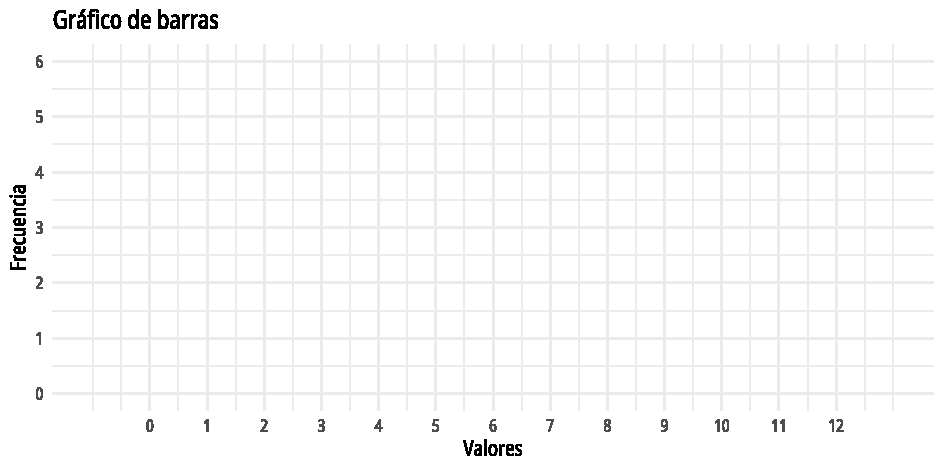
\includegraphics{grafico_vacio_013.pdf}\end{center}

\section*{Soluciones}
\setcounter{subsection}{0}
\subsection{}

\begin{center}\begin{tblr}{colspec={ccccc},hlines,vlines,hline{2,Z} = {1}{-}{},hline{2,Z} = {2}{-}{},row{even}={black!10}}
  .&Frecuencia&Probabilidad&Frecuencia Acumulada&Probabilidad Acumulada \\
 1&2&0.05&2&0.05 \\
 2&2&0.05&4&0.1 \\
 3&2&0.05&6&0.15 \\
 4&2&0.05&8&0.2 \\
 5&4&0.1&12&0.3 \\
 6&2&0.05&14&0.35 \\
 7&5&0.125&19&0.475 \\
 8&6&0.15&25&0.625 \\
 9&5&0.125&30&0.75 \\
 10&3&0.075&33&0.825 \\
 11&6&0.15&39&0.975 \\
 12&1&0.025&40&1 \\
 \end{tblr}\end{center}
\subsection{}
\begin{center}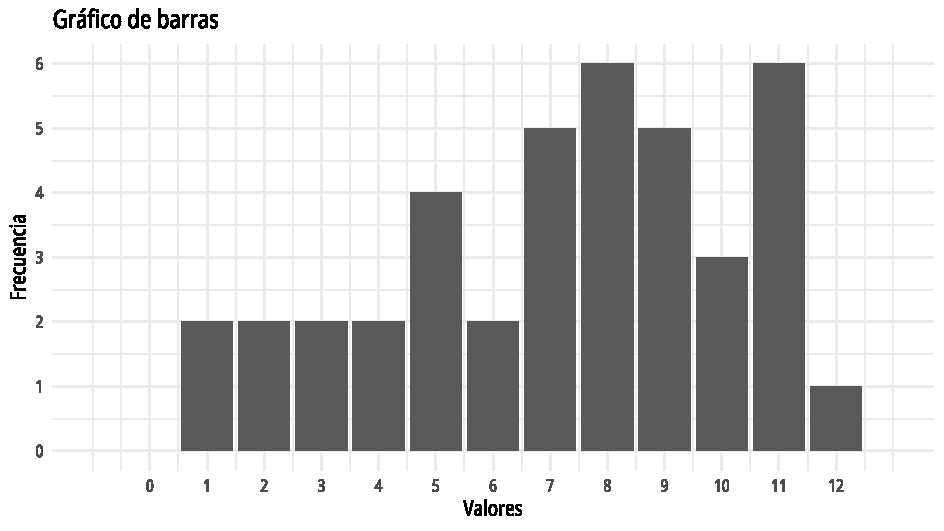
\includegraphics{grafico_barras_013.pdf}\end{center}
\end{document}
